%=================================================================
%\section{Unsupervised expansion of ad-hoc abbreviations in EHR narratives}

%-----------------------------------------------------------------
%\subsection{Materials and Methods}

\begin{frame}
	\frametitle{Materials and Methods}
	\begin{itemize} \myspacing
		\item 30,000 clinical documents from the cardiology domain
		\begin{itemize}
			\item Written in German by Austrian physicians
			\item Discharge summaries, finding reports        
                         \item Routine documentation in LKH, Graz
                \end{itemize}
                \item Evaluation data
                \begin{itemize}
                		\item Random subsequences of 100 characters
			\item 147 abbreviations manually expanded by a human annotator
                \end{itemize}
                \item Unsupervised machine learning
                \begin{itemize}
			\item Bigram and unigram lookup
			\item Training-test split (90\% - 10\%)
			\item Evaluated by accuracy
                \end{itemize}
	\end{itemize}
\end{frame}

\begin{frame}
	\frametitle{Materials and Methods}
                \begin{figure}
        			\centering
        			%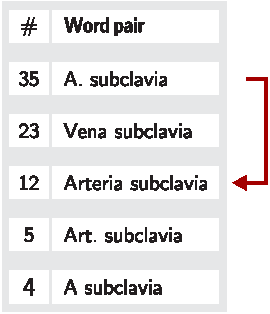
\includegraphics[width=10cm]{bigram_lookup.pdf}
        			\caption{Bigram lookup.}
        			\label{fig:bigram_lookup}
  		\end{figure}
\end{frame}

%-----------------------------------------------------------------


